\begin{figure}[htbp]
  \centering
  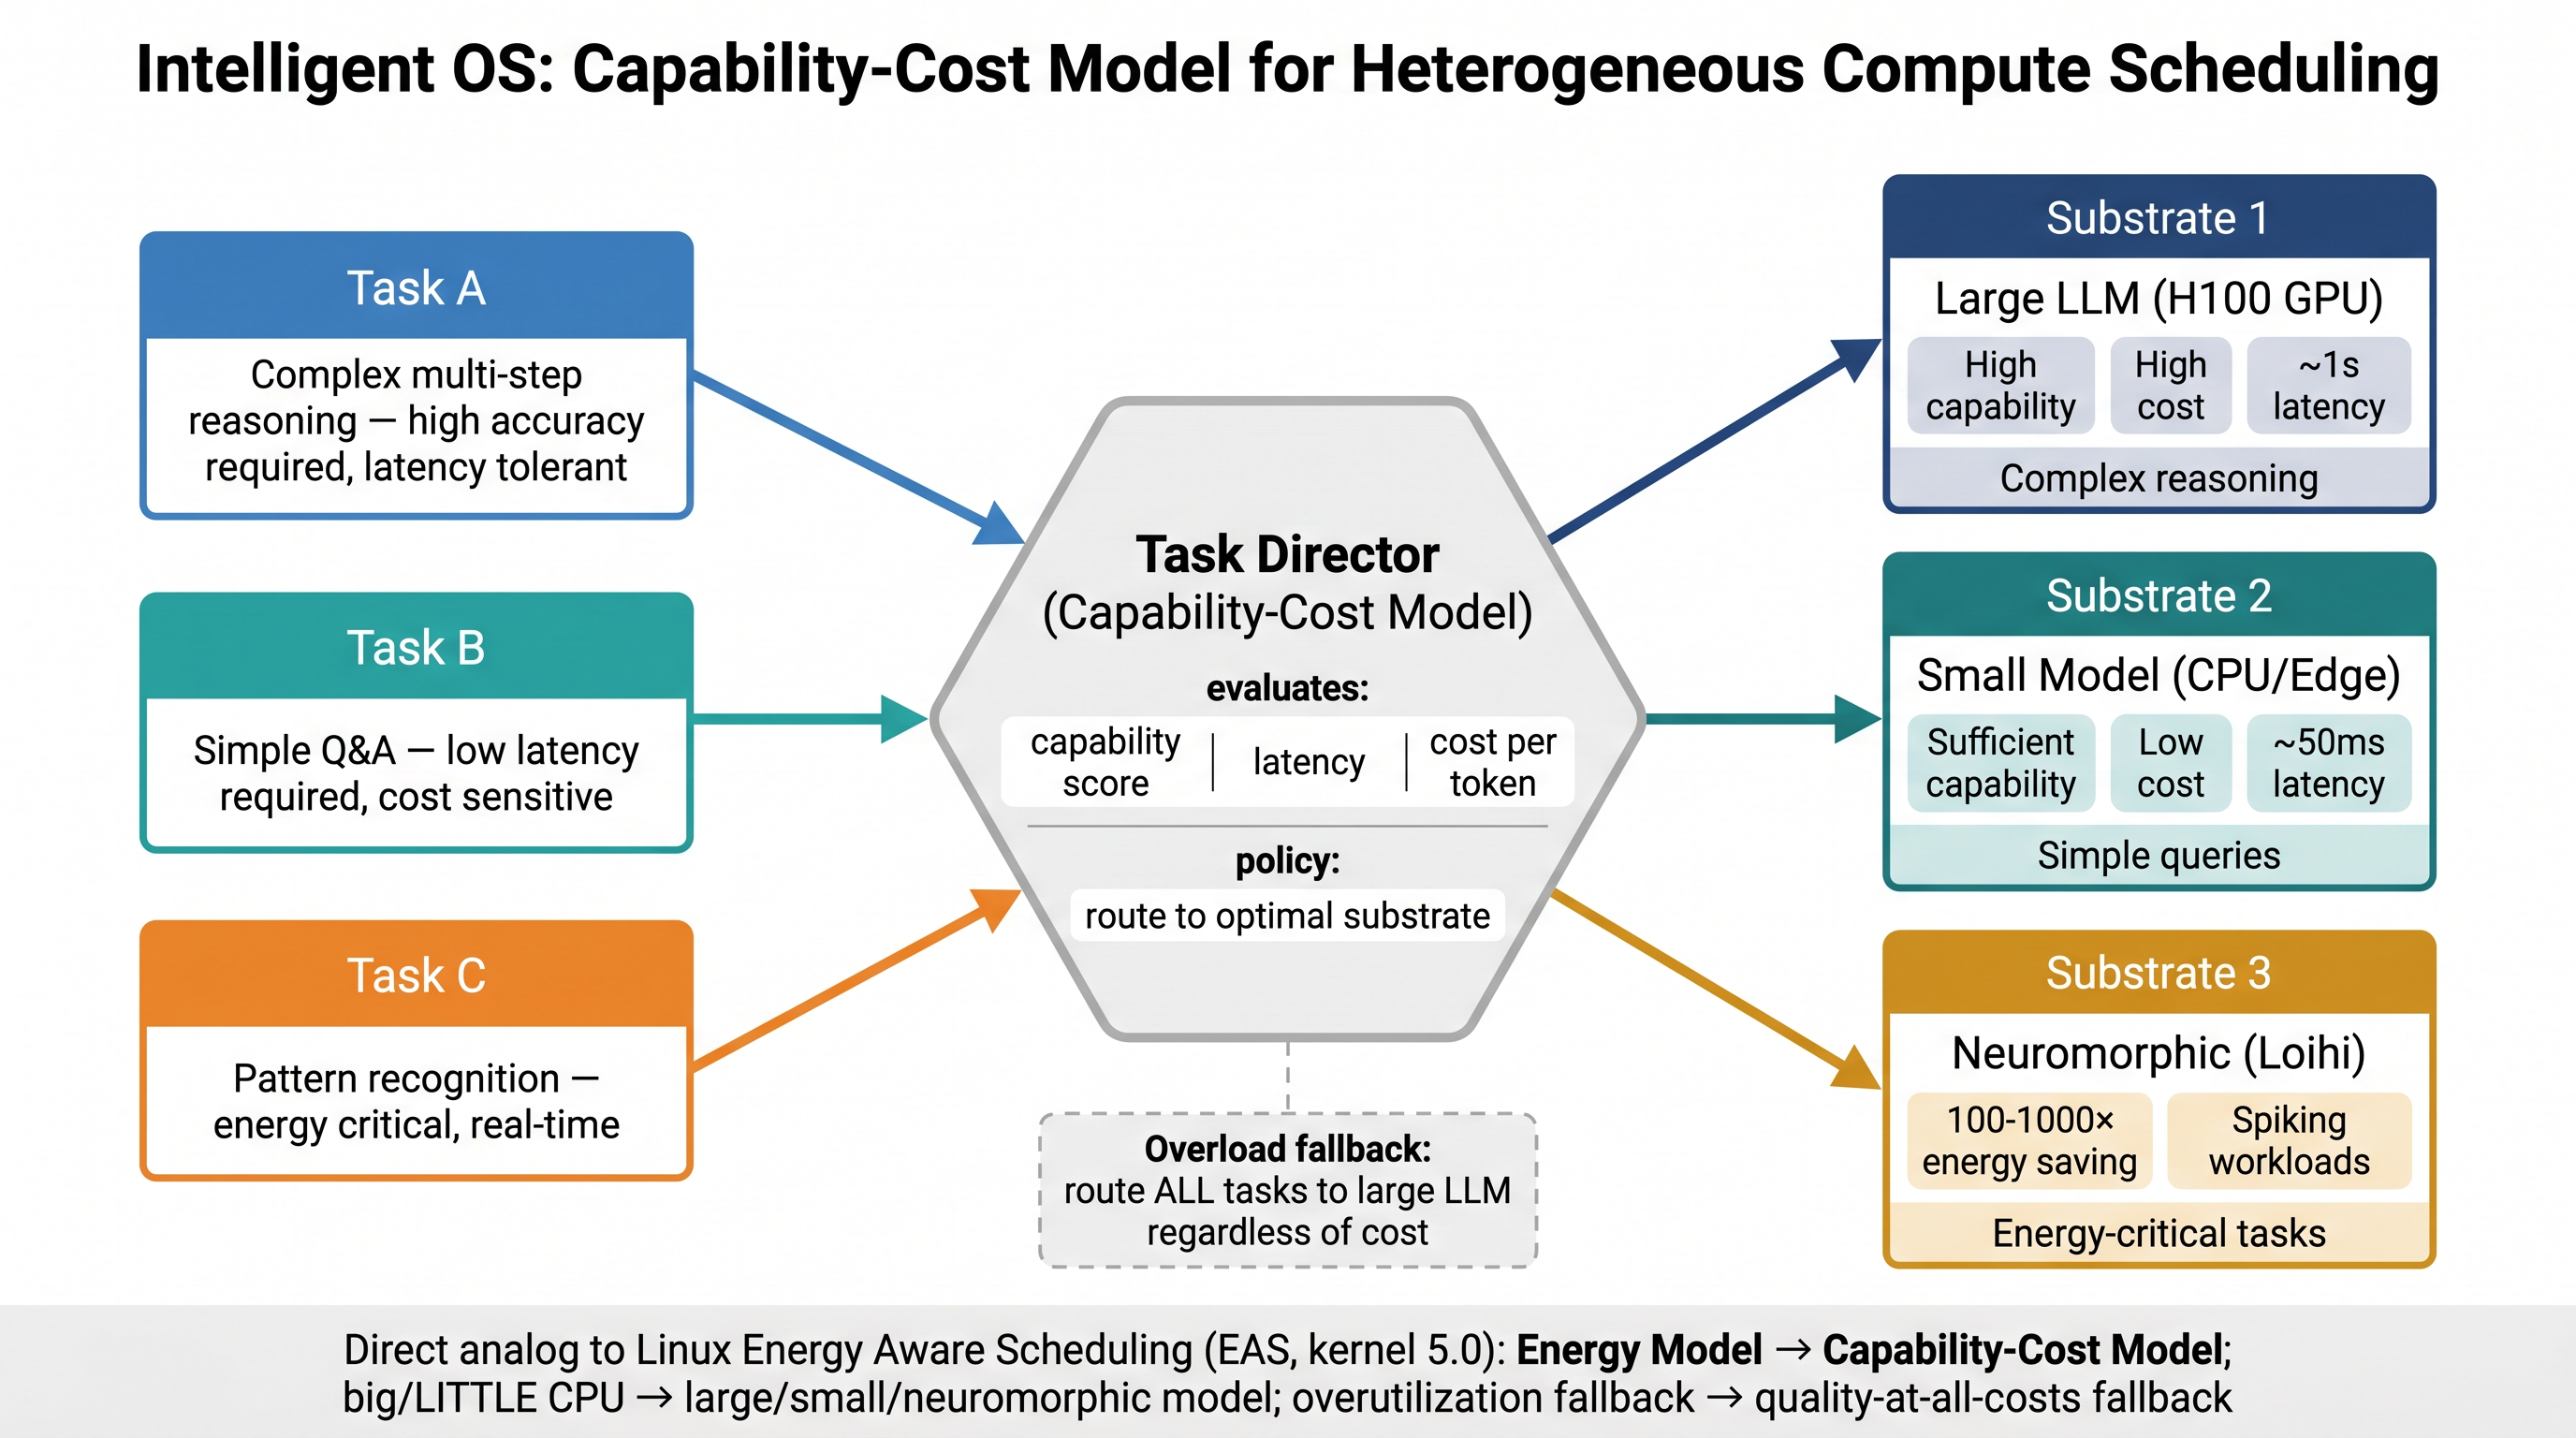
\includegraphics[width=0.88\textwidth]{figures/generated/fig_paradigm_scheduling}
  \caption{OS-level heterogeneous scheduling: Linux Energy Aware Scheduling (EAS) versus the intelligent OS Capability-Cost Model.
  EAS (Linux 5.0, 2019) uses an Energy Model to route each task to the most energy-efficient capable CPU
  and falls back to load balancing under overutilization.
  The Capability-Cost Model is the direct analog: a Task Director routes each subtask to
  the optimal compute core (large model, small model, neuromorphic, or biological substrate)
  by predicted capability, latency, and cost, falling back to the highest-capability core under peak load.}
  \label{fig:paradigm:scheduling}
\end{figure}
